% 第3章第2节：最小生成树（问题与最短路树的区别、割性质与安全选边、Kruskal、Prim、方法比较与结果检验）。

\section{最小生成树}
\label{sec:graph-minimum-spanning-tree}

要在若干城镇之间修路，使任意两个城镇都能互相到达，每条候选道路都有建造成本。这时关心的不是某两点之间怎样走最近，而是整张网络的总造价。第~\ref{sec:graph-trees-forests}节说明，连通且无环的边集恰好连接全部顶点而没有多余的边，即生成树；多一条边便形成环，环上任意一条边都可以拆掉而不破坏连通。于是问题化为：在所有生成树中找总边权最小的一棵。

本节先给出问题并与最短路区分，再建立割性质，它说明怎样的边可以放心地选入。Kruskal算法与Prim算法以不同的方式维护当前选边，但每一步都由割性质保证安全。最后在同一算例上比较两种算法，并区分“结果是一棵生成树”与“结果是最优的”这两种检查。

\subsection{最小生成树问题}
\label{sec:graph-opt-mst-problem}

设$\mathcal G=(V,E)$是有限无向连通图，每条边$e$带有实数权$w_e$，表示建造成本。对生成树$T\subseteq E$，记其总成本为$w(T)=\sum_{e\in T}w_e$。

\begin{definition}[最小生成树]
\label{def:graph-opt-mst}
有限无向连通加权图的所有生成树中，总成本$w(T)$最小者称为\term{最小生成树}（minimum spanning tree）。
\end{definition}

生成树只有有限多棵，所以最小生成树总是存在。它最小化的是连接全部顶点的总成本，并不保证树上每对顶点之间的路线都是原图中的最短路。图~\ref{fig:graph-opt-mst-vs-spt}中，三角形三条边的权为$w_{x,y}=2$、$w_{y,z}=2$、$w_{x,z}=3$。最小生成树取$\{xy,yz\}$，成本$4$；但在树上$x$到$z$要绕经$y$，长度为$4$，而原图中的直达边只有$3$。以$x$为源的\term{最短路树}（shortest-path tree），即由各顶点最短路的前驱弧组成的树，是$\{xy,xz\}$，成本$5$。两者回答不同的问题，一般不相同。同样，第~\ref{sec:graph-connectivity-computation}节由遍历得到的生成森林只保证连通与无环，不带有任何成本上的最优性。

\begin{figure}[!htb]
  \centering
  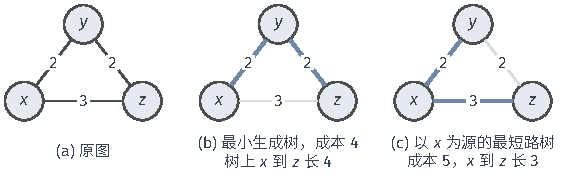
\includegraphics[width=95.793mm]{figures/01-basic-mathematics/04-graphs/tikz/c3-mst-vs-spt/figure.pdf}
  \caption{最小生成树与最短路树可以不同。(a) 原图，边旁为权。(b) 最小生成树$\{xy,yz\}$总成本$4$，但树上$x$到$z$的路线长$4$。(c) 以$x$为源的最短路树$\{xy,xz\}$保证每个顶点到$x$的距离最短，总成本却是$5$。蓝色粗边为所选的边。}
  \label{fig:graph-opt-mst-vs-spt}
\end{figure}

\paragraph{非连通、负权与平局}
图不连通时不存在生成树，问题改为在每个连通分量内分别求最小生成树，合起来称为\term{最小生成森林}（minimum spanning forest）。负权不会带来最短路那样的困难：每棵生成树恰有$n-1$条边，把所有边权同时加上常数$c$，每棵生成树的成本都增加$(n-1)c$，比较结果不变，因此总可以设想权都为正。边权有相同值时，最小生成树可能不止一棵，但最小总成本是唯一的。若要最大化总权，把全部边权取负即化为最小化问题，得到\term{最大生成树}（maximum spanning tree），下面的割性质与两种算法只需把“最小”改为“最大”即可照用。第~\ref{sec:graph-tree-decomposition-construction}节构造团树时会用到最大生成树。

\subsection{割性质与安全选边}
\label{sec:graph-opt-cut-property}

两种算法都是逐条选边，并希望每一步都不走错。“不走错”的确切含义是：当前已选的边集$A$总能扩充成某一棵最小生成树。只要保持这个不变量，选满$n-1$条边时，$A$本身就是一棵最小生成树。问题在于，下一条边选哪条才能保持不变量。

\paragraph{割与轻边}
把顶点集分成两个非空部分$S$与$V\setminus S$，称为图的一个\term{割}（cut），记作$(S,V\setminus S)$。一条边的两个端点分别在两侧时，称它跨越这个割。若已选边集$A$中没有边跨越该割，就称这个割与$A$相容。跨越某个割的边中权最小的称为该割的\term{轻边}（light edge），权相同时轻边可以不止一条。

\begin{lemma}[割性质]
\label{lem:graph-opt-cut-property}
设$\mathcal G$是有限无向连通加权图，边集$A$包含在某棵最小生成树中，割$(S,V\setminus S)$与$A$相容，$e$是该割的一条轻边。则$A\cup\{e\}$也包含在某棵最小生成树中。
\end{lemma}

\begin{proof}
取一棵包含$A$的最小生成树$T$。若$e\in T$，结论已成立。否则把$e$加入$T$，由第~\ref{sec:graph-trees-forests}节，树加一条边恰好形成一个环。设$e=\{u,v\}$，$u\in S$、$v\notin S$，这个环由$e$与$T$中$u$到$v$的路径组成。这条路径从$S$出发，最终到达$V\setminus S$，所以其中至少有一条边$f$跨越该割。

从$T+e$中删去$f$，环被打断，所得边集$T'=T+e-f$仍连通且有$n-1$条边，因而是生成树。由于$e$是轻边，$w_e\leq w_f$，所以$w(T')=w(T)+w_e-w_f\leq w(T)$，$T'$也是最小生成树。最后，割与$A$相容，跨越割的$f$不在$A$中，删去$f$不影响$A$；于是$A\cup\{e\}\subseteq T'$。
\end{proof}

图~\ref{fig:graph-opt-cut-exchange}画出这一交换：轻边$e$加入后与树中路径形成环，环上另一条跨割边$f$被删去，成本不增。

\begin{figure}[!htb]
  \centering
  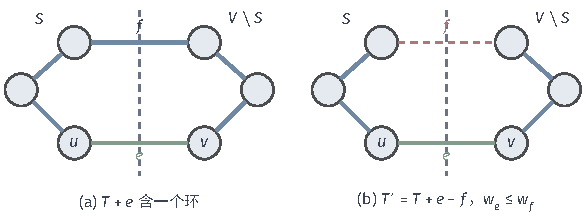
\includegraphics[width=99.187mm]{figures/01-basic-mathematics/04-graphs/tikz/c3-cut-exchange/figure.pdf}
  \caption{割性质的交换论证。虚线把顶点分成$S$与$V\setminus S$，蓝色粗边为最优树$T$，其中不跨割的边包含当前选边$A$。(a) 轻边$e$（绿色）不在$T$中，加入后与$T$中$u$到$v$的路径形成环。(b) 环上另一条跨割边$f$（红色虚线）被删去，得到$T'=T+e-f$，因$w_e\leq w_f$，成本不增。}
  \label{fig:graph-opt-cut-exchange}
\end{figure}

\paragraph{安全不等于必选}
割性质只保证轻边能留在\emph{某一棵}最优树中，并不保证它出现在\emph{每一棵}最优树中。设三角形三条边的权都是$1$，取割$(\{x\},\{y,z\})$，$xy$与$xz$都是轻边。最小生成树$\{xy,yz\}$不含$xz$，但按割性质选入$xz$仍然安全，因为$\{xz,yz\}$同样是最小生成树。平局时不同的选择通向不同的最优树，最优成本却相同。

割性质是两种算法的共同依据，区别只在于它们选取哪个割：Kruskal算法以当前森林中某个分量作为$S$，Prim算法以当前唯一一棵树的顶点集作为$S$。

\subsection{Kruskal算法}
\label{sec:graph-opt-kruskal}

一种自然的想法是从最便宜的边开始逐条考虑，只要不形成环就选入。开始时每个顶点自成一个分量；一条边的两端若属于不同分量，选入它会把两个分量连起来，不会成环；若两端已在同一分量，选入它就会成环，应当跳过。

\begin{algorithm}[Kruskal算法]
\label{alg:graph-opt-kruskal}
输入：有限无向加权图。输出：最小生成森林的边集$A$。状态：已选边集$A$与维护当前分量的并查集。
\begin{enumerate}
  \item 令$A=\varnothing$，为每个顶点建立一个单元素集合；把全部边按权从小到大排序，平局按固定的边序。
  \item 按排序依次取边$\{u,v\}$：若$u,v$的代表不同，把这条边加入$A$并合并两个集合；若代表相同，跳过。
  \item 选满$n-1$条边时可提前停止；否则扫描完全部边，输出的$A$是最小生成森林，集合个数即连通分量数。
\end{enumerate}
\end{algorithm}

判断两端是否属于同一分量、以及合并两个分量，正是第~\ref{sec:graph-connectivity-computation}节并查集的find与union操作。每选一条边，分量数减一且不产生环，所以选边数加分量数始终等于$n$。

\paragraph{算例}
取五个顶点$a,b,c,d,e$与七条边，权为$ab=1$、$bc=2$、$cd=3$、$ac=4$、$bd=5$、$ce=6$、$de=7$。按权依次考虑：$ab$、$bc$、$cd$的两端都属于不同分量，依次选入，此时分量为$\{a,b,c,d\}$与$\{e\}$，累计成本$6$；$ac$与$bd$的两端都已在$\{a,b,c,d\}$中，选入会成环，跳过；$ce$连接两个分量，选入后只剩一个分量，已选满$4=n-1$条边，停止。结果为$\{ab,bc,cd,ce\}$，总成本$1+2+3+6=12$。图~\ref{fig:graph-opt-kruskal-steps}画出了这一过程。这个图共有$21$棵生成树，逐一枚举可以核对成本$12$的只有这一棵，次优的成本为$13$。

\begin{figure}[!htb]
  \centering
  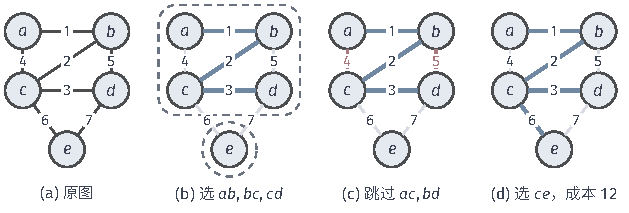
\includegraphics[width=106.5mm]{figures/01-basic-mathematics/04-graphs/tikz/c3-kruskal-steps/figure.pdf}
  \caption{Kruskal算法在五点七边图上的过程。(a) 原图，边旁为权。(b) 依次选入$ab,bc,cd$（蓝色粗边），虚线框标出当前分量$\{a,b,c,d\}$与$\{e\}$。(c) $ac$与$bd$的两端已在同一分量，选入会成环，跳过（红色虚线）。(d) 选入$ce$，得到最小生成树$\{ab,bc,cd,ce\}$，总成本$12$。}
  \label{fig:graph-opt-kruskal-steps}
\end{figure}

\paragraph{正确性}
下面用割性质说明Kruskal算法每次选入的边都是安全的。

\begin{theorem}[Kruskal算法的正确性]
\label{thm:graph-opt-kruskal}
对有限无向加权图，算法~\ref{alg:graph-opt-kruskal}输出一个最小生成森林；图连通时输出最小生成树。
\end{theorem}

\begin{proof}
先设图连通，证明不变量“$A$包含在某棵最小生成树中”。初始$A=\varnothing$，结论成立。设算法即将选入边$e=\{u,v\}$，取$S$为森林$(V,A)$中$u$所在的分量，则$v\notin S$，割$(S,V\setminus S)$与$A$相容。考察任意一条跨越这个割、权小于$w_e$的边$g$。它排在$e$之前，已被处理过：若当时被选入，它就在$A$中，而$A$中没有跨割的边；若当时被跳过，它的两端当时已在同一分量，分量只会合并而不会拆开，现在仍在同一分量，也不能跨割。所以跨越该割的边权都不小于$w_e$，$e$是轻边，由引理~\ref{lem:graph-opt-cut-property}，选入$e$后不变量仍成立。

扫描结束时，若原图中某条边连接了$(V,A)$的两个不同分量，处理到它时两端必属不同分量，它就会被选入，矛盾。所以$(V,A)$的分量与原图的分量相同，图连通时$A$是生成树。它包含在某棵最小生成树中，又与之边数相同，因而本身就是最小生成树。图不连通时，对每个分量分别应用上面的论证，结论对最小生成森林同样成立。
\end{proof}

\paragraph{计算开销}
排序需要$O(m\log m)$时间。之后至多处理$m$条边，每条边做两次find，选入时再做一次union，共$O(m)$次并查集操作。采用第~\ref{sec:graph-connectivity-computation}节的按大小合并时，树高不超过$O(\log n)$，每次操作$O(\log n)$，这部分为$O(m\log n)$；由于$m\leq n^2$，$\log m\leq2\log n$，总时间为$O(m\log n)$，空间为边表与并查集的$O(n+m)$。若再配合路径压缩，并查集操作的摊还开销几乎为常数，此时排序成为主要开销。算法的正确性只依赖割性质，与并查集采用哪种实现无关。

\subsection{Prim算法}
\label{sec:graph-opt-prim}

Kruskal算法同时维护许多分量，按全局次序选边。另一种做法是只让一棵树生长：从一个顶点出发，每次把一个外部顶点用最便宜的边接到树上。

\paragraph{键与算法步骤}
为每个尚未入树的顶点$v$记录一个键$\operatorname{key}(v)$，表示$v$与当前树之间最便宜的边的权，同时记录这条边在树内的端点$p(v)$。这里的键是\emph{一条}连接边的权，不是Dijkstra算法中从源点出发的累计长度。

\begin{algorithm}[Prim算法]
\label{alg:graph-opt-prim}
输入：有限无向连通加权图、起点$r$。输出：最小生成树的边集。状态：树的顶点集$S$、外部顶点的键与父点、按键排序的优先队列。
\begin{enumerate}
  \item 令$S=\{r\}$；对$r$的每个邻居$v$，令$\operatorname{key}(v)=w_{r,v}$、$p(v)=r$，其余外部顶点的键为$+\infty$。
  \item 当$S\neq V$时，取出键最小的外部顶点$u$，把$u$加入$S$，把边$\{p(u),u\}$加入树。
  \item 对$u$的每个外部邻居$v$，若$w_{u,v}<\operatorname{key}(v)$，令$\operatorname{key}(v)=w_{u,v}$、$p(v)=u$。
\end{enumerate}
\end{algorithm}

第三步之后，每个外部顶点的键仍等于它与$S$中顶点之间最便宜的边权：新加入的$u$只带来了从$u$出发的边，逐一比较即可。因此每次取出的最小键对应的边，正是割$(S,V\setminus S)$的一条轻边。

\paragraph{算例}
在与Kruskal算法相同的五点图上从$a$出发，过程如图~\ref{fig:graph-opt-prim-steps}。开始时$\operatorname{key}(b)=1$、$\operatorname{key}(c)=4$。取出$b$，选入$ab$；$b$的邻边把$c$的键从$4$改为$2$，并给$d$设键$5$。取出$c$，选入$bc$；$d$的键从$5$改为$3$，$e$得到键$6$。取出$d$，选入$cd$；$de=7$不优于$e$现有的键$6$，不更新。最后取出$e$，选入$ce$。所得的树与Kruskal算法相同，成本$12$。

\begin{figure*}[!htb]
  \centering
  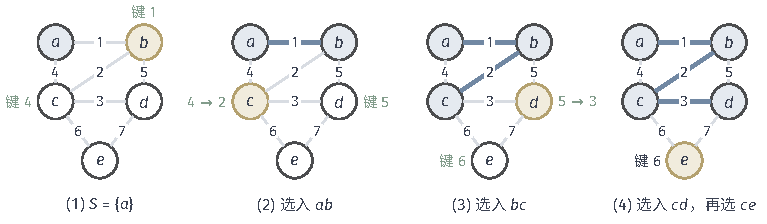
\includegraphics[width=129.858mm]{figures/01-basic-mathematics/04-graphs/tikz/c3-prim-steps/figure.pdf}
  \caption{Prim算法从$a$出发的过程。每个面板中蓝色顶点与蓝色粗边是当前树，外部顶点旁标出键，绿色表示刚被改善的键，黄色为下一个取出的顶点。依次选入$ab,bc,cd,ce$，各步加入的边恰是当前树顶点集所形成割的轻边；最终的树与Kruskal算法相同，成本$12$。}
  \label{fig:graph-opt-prim-steps}
\end{figure*}

换一个起点，选边次序会变。从$e$出发时，$c$与$d$的键分别为$6$与$7$；先选入$ec=6$，$c$的邻边使$b$、$a$、$d$的键变为$2$、$4$、$3$；再选入$cb=2$，$a$的键降为$1$；随后选入$ba=1$与$cd=3$。所选边权依次为$6,2,1,3$，并不递增。这与Kruskal算法的全局排序不同：Prim算法每次只在当前割上取最轻的边，不同时刻面对的是不同的割。

\paragraph{正确性}
正确性同样来自割性质：令$A$为当前树的边集，$S$为其顶点集。$A$的边都在$S$内部，割$(S,V\setminus S)$与$A$相容；算法选入的边是该割的轻边，由引理~\ref{lem:graph-opt-cut-property}，若$A$包含在某棵最小生成树中，加入新边后仍然如此。从$A=\varnothing$出发归纳，选满$n-1$条边时得到最小生成树。

\paragraph{实现与开销}
用数组保存键、每次线性扫描找最小时，$n$次取最小共$O(n^2)$，每条边至多引起一次键的比较与更新，总时间为$O(n^2+m)$，适合稠密图。用支持降键的索引二叉堆时，取最小与降键各需$O(\log n)$，总时间为$O((n+m)\log n)$，适合稀疏图。两种实现的额外空间都是$O(n)$。图不连通时，一棵树长满所在分量后，从任一尚未访问的顶点重新开始，得到最小生成森林，各分量的父边与成本分别保留。

\subsection{方法比较与结果检验}
\label{sec:graph-opt-mst-comparison}

两种算法读取边与维护状态的方式不同。Kruskal算法一次性对全部边排序，按全局次序检查，用并查集维护多个分量，适合边已经以列表形式给出的稀疏图。Prim算法从一棵树出发，只读取新入树顶点的邻边，用键数组或堆维护局部信息，在用邻接矩阵存储的稠密图上，数组版本的$O(n^2)$开销已与读入图的开销同阶。孰优孰劣取决于图的稠密程度、边的组织方式和所用数据结构，不能只凭算法名称判断。

\paragraph{可行性与最优性}
检验一份声称的最小生成森林时，先确认它是一个可行的生成森林：所选的每条边都来自原图；每个原连通分量的顶点都被覆盖；所选边无环，可以用并查集逐条加入核对；选边数等于$n$减去分量数。然后重算总成本。这些检查只证明结果是\emph{一个}生成森林，不能证明它最优。

最优性要回到割性质与算法的交换论证。一种可以独立执行的检查是：对每条未被选中的边$\{u,v\}$，考察树上$u$到$v$的路径，若路径上有一条边的权大于$w_{u,v}$，用这条非树边替换它，就得到成本更低的生成树，结果必不最优。反过来，若每条非树边都不轻于它在树上对应路径中的每条边，这棵树就是最优的；这一充分性可以仿照割性质的交换论证证明，这里从略。小规模的例子还可以枚举全部生成树作对照，如前面的五点图。但两种算法在某个例子上给出相同的树，只是一致性的旁证，不能当作一般正确性的证明。
